% Options for packages loaded elsewhere
\PassOptionsToPackage{unicode}{hyperref}
\PassOptionsToPackage{hyphens}{url}
%
\documentclass[
]{article}
\usepackage{amsmath,amssymb}
\usepackage{iftex}
\ifPDFTeX
  \usepackage[T1]{fontenc}
  \usepackage[utf8]{inputenc}
  \usepackage{textcomp} % provide euro and other symbols
\else % if luatex or xetex
  \usepackage{unicode-math} % this also loads fontspec
  \defaultfontfeatures{Scale=MatchLowercase}
  \defaultfontfeatures[\rmfamily]{Ligatures=TeX,Scale=1}
\fi
\usepackage{lmodern}
\ifPDFTeX\else
  % xetex/luatex font selection
\fi
% Use upquote if available, for straight quotes in verbatim environments
\IfFileExists{upquote.sty}{\usepackage{upquote}}{}
\IfFileExists{microtype.sty}{% use microtype if available
  \usepackage[]{microtype}
  \UseMicrotypeSet[protrusion]{basicmath} % disable protrusion for tt fonts
}{}
\makeatletter
\@ifundefined{KOMAClassName}{% if non-KOMA class
  \IfFileExists{parskip.sty}{%
    \usepackage{parskip}
  }{% else
    \setlength{\parindent}{0pt}
    \setlength{\parskip}{6pt plus 2pt minus 1pt}}
}{% if KOMA class
  \KOMAoptions{parskip=half}}
\makeatother
\usepackage{xcolor}
\usepackage[margin=1in]{geometry}
\usepackage{color}
\usepackage{fancyvrb}
\newcommand{\VerbBar}{|}
\newcommand{\VERB}{\Verb[commandchars=\\\{\}]}
\DefineVerbatimEnvironment{Highlighting}{Verbatim}{commandchars=\\\{\}}
% Add ',fontsize=\small' for more characters per line
\usepackage{framed}
\definecolor{shadecolor}{RGB}{248,248,248}
\newenvironment{Shaded}{\begin{snugshade}}{\end{snugshade}}
\newcommand{\AlertTok}[1]{\textcolor[rgb]{0.94,0.16,0.16}{#1}}
\newcommand{\AnnotationTok}[1]{\textcolor[rgb]{0.56,0.35,0.01}{\textbf{\textit{#1}}}}
\newcommand{\AttributeTok}[1]{\textcolor[rgb]{0.13,0.29,0.53}{#1}}
\newcommand{\BaseNTok}[1]{\textcolor[rgb]{0.00,0.00,0.81}{#1}}
\newcommand{\BuiltInTok}[1]{#1}
\newcommand{\CharTok}[1]{\textcolor[rgb]{0.31,0.60,0.02}{#1}}
\newcommand{\CommentTok}[1]{\textcolor[rgb]{0.56,0.35,0.01}{\textit{#1}}}
\newcommand{\CommentVarTok}[1]{\textcolor[rgb]{0.56,0.35,0.01}{\textbf{\textit{#1}}}}
\newcommand{\ConstantTok}[1]{\textcolor[rgb]{0.56,0.35,0.01}{#1}}
\newcommand{\ControlFlowTok}[1]{\textcolor[rgb]{0.13,0.29,0.53}{\textbf{#1}}}
\newcommand{\DataTypeTok}[1]{\textcolor[rgb]{0.13,0.29,0.53}{#1}}
\newcommand{\DecValTok}[1]{\textcolor[rgb]{0.00,0.00,0.81}{#1}}
\newcommand{\DocumentationTok}[1]{\textcolor[rgb]{0.56,0.35,0.01}{\textbf{\textit{#1}}}}
\newcommand{\ErrorTok}[1]{\textcolor[rgb]{0.64,0.00,0.00}{\textbf{#1}}}
\newcommand{\ExtensionTok}[1]{#1}
\newcommand{\FloatTok}[1]{\textcolor[rgb]{0.00,0.00,0.81}{#1}}
\newcommand{\FunctionTok}[1]{\textcolor[rgb]{0.13,0.29,0.53}{\textbf{#1}}}
\newcommand{\ImportTok}[1]{#1}
\newcommand{\InformationTok}[1]{\textcolor[rgb]{0.56,0.35,0.01}{\textbf{\textit{#1}}}}
\newcommand{\KeywordTok}[1]{\textcolor[rgb]{0.13,0.29,0.53}{\textbf{#1}}}
\newcommand{\NormalTok}[1]{#1}
\newcommand{\OperatorTok}[1]{\textcolor[rgb]{0.81,0.36,0.00}{\textbf{#1}}}
\newcommand{\OtherTok}[1]{\textcolor[rgb]{0.56,0.35,0.01}{#1}}
\newcommand{\PreprocessorTok}[1]{\textcolor[rgb]{0.56,0.35,0.01}{\textit{#1}}}
\newcommand{\RegionMarkerTok}[1]{#1}
\newcommand{\SpecialCharTok}[1]{\textcolor[rgb]{0.81,0.36,0.00}{\textbf{#1}}}
\newcommand{\SpecialStringTok}[1]{\textcolor[rgb]{0.31,0.60,0.02}{#1}}
\newcommand{\StringTok}[1]{\textcolor[rgb]{0.31,0.60,0.02}{#1}}
\newcommand{\VariableTok}[1]{\textcolor[rgb]{0.00,0.00,0.00}{#1}}
\newcommand{\VerbatimStringTok}[1]{\textcolor[rgb]{0.31,0.60,0.02}{#1}}
\newcommand{\WarningTok}[1]{\textcolor[rgb]{0.56,0.35,0.01}{\textbf{\textit{#1}}}}
\usepackage{graphicx}
\makeatletter
\def\maxwidth{\ifdim\Gin@nat@width>\linewidth\linewidth\else\Gin@nat@width\fi}
\def\maxheight{\ifdim\Gin@nat@height>\textheight\textheight\else\Gin@nat@height\fi}
\makeatother
% Scale images if necessary, so that they will not overflow the page
% margins by default, and it is still possible to overwrite the defaults
% using explicit options in \includegraphics[width, height, ...]{}
\setkeys{Gin}{width=\maxwidth,height=\maxheight,keepaspectratio}
% Set default figure placement to htbp
\makeatletter
\def\fps@figure{htbp}
\makeatother
\setlength{\emergencystretch}{3em} % prevent overfull lines
\providecommand{\tightlist}{%
  \setlength{\itemsep}{0pt}\setlength{\parskip}{0pt}}
\setcounter{secnumdepth}{-\maxdimen} % remove section numbering
\usepackage{transparent}
\usepackage[utf8]{inputenx}
\usepackage{iwona}
\usepackage{tikz}
\usepackage{dcolumn}
\usepackage{color}
\usepackage[italian]{babel}
\usepackage{listings}
\usepackage{hyperref}
\usepackage{setspace}
\usepackage{enumitem}
\usepackage{tocloft}
\usepackage{eso-pic}
\geometry{verbose,tmargin=5cm,bmargin=3.5cm,lmargin=2.5cm,rmargin=2.5cm}
\ifLuaTeX
  \usepackage{selnolig}  % disable illegal ligatures
\fi
\IfFileExists{bookmark.sty}{\usepackage{bookmark}}{\usepackage{hyperref}}
\IfFileExists{xurl.sty}{\usepackage{xurl}}{} % add URL line breaks if available
\urlstyle{same}
\hypersetup{
  pdftitle={Homework \#01},
  pdfauthor={SMDS-2023-2024},
  hidelinks,
  pdfcreator={LaTeX via pandoc}}

\title{Homework \#01}
\author{SMDS-2023-2024}
\date{\textsc{\textbf{\Large Statstical Methods in Data Science II a.y. 2022-2023}}\\
\strut \\
M.Sc. in Data Science\\
\strut \\
\underline{deadline: April 26th, 2024}}

\begin{document}
\maketitle

\hypertarget{a.-simulation}{%
\subsection{A. Simulation}\label{a.-simulation}}

\hypertarget{consider-the-following-joint-discrete-distribution-of-a-random-vector-yz-taking-values-over-the-bi-variate-space}{%
\subsubsection{\texorpdfstring{1. Consider the following joint discrete
distribution of a random vector \((Y,Z)\) taking values over the
bi-variate
space:}{1. Consider the following joint discrete distribution of a random vector (Y,Z) taking values over the bi-variate space:}}\label{consider-the-following-joint-discrete-distribution-of-a-random-vector-yz-taking-values-over-the-bi-variate-space}}

\begin{eqnarray*}
{\cal S} = {\cal Y} \times {\cal Z} &=& \{(1,1);(1,2);(1,3);\\
&& (2,1);(2,2);(2,3);\\
&& (3,1);(3,2);(3,3)\}
\end{eqnarray*} The joint probability distribution is provided as a
matrix \(\texttt{J}\) whose generic entry
\(\texttt{J[y,z]}=Pr \{Y=y,Z=z\}\)

\begin{Shaded}
\begin{Highlighting}[]
\NormalTok{J}
\end{Highlighting}
\end{Shaded}

\begin{verbatim}
     1    2    3
1 0.06 0.17 0.10
2 0.10 0.12 0.11
3 0.14 0.02 0.18
\end{verbatim}

\begin{Shaded}
\begin{Highlighting}[]
\NormalTok{S}
\end{Highlighting}
\end{Shaded}

\begin{verbatim}
      row col
(1,1)   1   1
(1,2)   1   2
(1,3)   1   3
(2,1)   2   1
(2,2)   2   2
(2,3)   2   3
(3,1)   3   1
(3,2)   3   2
(3,3)   3   3
\end{verbatim}

You can load the matrix \texttt{S} of all the couples of the states in
\({\cal S}\) and the matrix \texttt{J} containing the corresponding
bivariate probability masses from the file ``Hmwk.RData''. How can you
check that \(J\) is a probability distribution?

\begin{center}\rule{0.5\linewidth}{0.5pt}\end{center}

\hypertarget{answer}{%
\subsubsection{1. Answer:}\label{answer}}

We can check whether \(J\) is a \emph{valid probability distribution} by
verifying if it satisfies the two properties of \emph{non-negativity}
and \emph{summation to 1}. Since \(J\) is discrete we will refer to the
discrete versions of the properties.

The first states that all elements of the probability distribution must
be non-negative:

\[
Pr \{Y=y,Z=z\} \ge 0 \; \forall y,z \in \{1, 2, 3\}
\]

We can write a simple conditional statement to check if this condition
is satisfied:

\begin{Shaded}
\begin{Highlighting}[]
\CommentTok{\# function to verify if a probability}
\CommentTok{\# distribution is non{-}negative}
\NormalTok{verify\_non\_negativity }\OtherTok{\textless{}{-}} \ControlFlowTok{function}\NormalTok{(A) \{}
    \FunctionTok{return}\NormalTok{(}\FunctionTok{sum}\NormalTok{(A }\SpecialCharTok{\textgreater{}=} \DecValTok{0}\NormalTok{) }\SpecialCharTok{==} \FunctionTok{length}\NormalTok{(A))}
\NormalTok{\}}

\FunctionTok{verify\_non\_negativity}\NormalTok{(J)}
\end{Highlighting}
\end{Shaded}

\begin{verbatim}
[1] TRUE
\end{verbatim}

As we can see the first property is satisfied. The property of summation
to 1 instead states that the elements of the probability distribution
must sum up to 1:

\[
\sum_{y,z \in \{ 1,2,3 \} } Pr \{ Y=y, Z=z \} = 1
\]

This also can be checked with a simple conditional statement:

\begin{Shaded}
\begin{Highlighting}[]
\CommentTok{\# function to verify is a probability}
\CommentTok{\# distribution has sum equal to 1}
\NormalTok{verify\_sum\_to\_one }\OtherTok{\textless{}{-}} \ControlFlowTok{function}\NormalTok{(A) \{}
    \FunctionTok{return}\NormalTok{(}\FunctionTok{all.equal}\NormalTok{(}\FunctionTok{sum}\NormalTok{(A), }\DecValTok{1}\NormalTok{))}
\NormalTok{\}}
\end{Highlighting}
\end{Shaded}

It's important to notice that, to account for \emph{machine precision},
we used the method \texttt{all.equal} instead of the \texttt{==}
operator.

\begin{Shaded}
\begin{Highlighting}[]
\FunctionTok{verify\_sum\_to\_one}\NormalTok{(J)}
\end{Highlighting}
\end{Shaded}

\begin{verbatim}
[1] TRUE
\end{verbatim}

Also the second condition is satisfied, therefore we can say that \(J\)
is indeed a valid probability distribution.

\begin{center}\rule{0.5\linewidth}{0.5pt}\end{center}

\hypertarget{how-many-conditional-distributions-can-be-derived-from-the-joint-distribution-j-please-list-and-derive-them.}{%
\subsubsection{\texorpdfstring{2. How many \emph{conditional
distributions} can be derived from the joint distribution \texttt{J}?
Please list and derive
them.}{2. How many conditional distributions can be derived from the joint distribution J? Please list and derive them.}}\label{how-many-conditional-distributions-can-be-derived-from-the-joint-distribution-j-please-list-and-derive-them.}}

\begin{center}\rule{0.5\linewidth}{0.5pt}\end{center}

\hypertarget{answer-1}{%
\subsubsection{2. Answer:}\label{answer-1}}

We can derive \(6\) conditional probability distributions by fixing on
either \(Y\) or \(Z\) a value in \(\{1,2,3\}\); we have \(2\) random
variables with \(3\) possible values each, therefore \(3*2=6\)
conditional distributions. To derive them we have just to implement the
definition of conditional probability:

\[
Pr(Y = y | Z = z) = \frac{Pr(Y = y, Z = z)}{Pr(Z = z)}
\]

Where at the numerator we have the joint distribution, provided by the
matrix \(J\), and at the denominator the \emph{marginal distribution} of
the value we condition on, defined as:

\[
Pr(Z = z) = \sum_y Pr(Y = y, Z = z)
\]

The base elements of this second formula are the joint distributions
that we already know, therefore we have derived all ingredients we need
for the computation. In the previous definitions \(Y\) and \(Z\) can be
swapped to get the formulas for \(Z\) conditioned on \(Y\). Below we
implement the functions to get the marginal and conditional
distributions:

\begin{Shaded}
\begin{Highlighting}[]
\CommentTok{\# support of y}
\NormalTok{Y }\OtherTok{=} \DecValTok{1}\SpecialCharTok{:}\DecValTok{3}
\CommentTok{\# support of z}
\NormalTok{Z }\OtherTok{=} \DecValTok{1}\SpecialCharTok{:}\DecValTok{3}

\CommentTok{\# marginal distribution of z}
\NormalTok{get\_marginal\_distro\_Z }\OtherTok{\textless{}{-}} \ControlFlowTok{function}\NormalTok{() \{}
\NormalTok{    marginal }\OtherTok{=} \FunctionTok{c}\NormalTok{()}
    \ControlFlowTok{for}\NormalTok{ (z }\ControlFlowTok{in} \DecValTok{1}\SpecialCharTok{:}\DecValTok{3}\NormalTok{) \{}
\NormalTok{        marginal }\OtherTok{=} \FunctionTok{c}\NormalTok{(marginal, }\FunctionTok{sum}\NormalTok{(J[, z]))}
\NormalTok{    \}}
    \FunctionTok{return}\NormalTok{(marginal)}
\NormalTok{\}}

\CommentTok{\# marginal distribution of y}
\NormalTok{get\_marginal\_distro\_Y }\OtherTok{\textless{}{-}} \ControlFlowTok{function}\NormalTok{() \{}
\NormalTok{    marginal }\OtherTok{=} \FunctionTok{c}\NormalTok{()}
    \ControlFlowTok{for}\NormalTok{ (y }\ControlFlowTok{in} \DecValTok{1}\SpecialCharTok{:}\DecValTok{3}\NormalTok{) \{}
\NormalTok{        marginal }\OtherTok{=} \FunctionTok{c}\NormalTok{(marginal, }\FunctionTok{sum}\NormalTok{(J[y, ]))}
\NormalTok{    \}}
    \FunctionTok{return}\NormalTok{(marginal)}
\NormalTok{\}}

\CommentTok{\# marginal distribution of y given z}
\NormalTok{get\_conditional\_distro\_Y }\OtherTok{\textless{}{-}} \ControlFlowTok{function}\NormalTok{(y, z) \{}
    \FunctionTok{return}\NormalTok{(J[y, z]}\SpecialCharTok{/}\FunctionTok{get\_marginal\_distro\_Z}\NormalTok{()[z])}
\NormalTok{\}}

\CommentTok{\# marginal distribution of z given y}
\NormalTok{get\_conditional\_distro\_Z }\OtherTok{\textless{}{-}} \ControlFlowTok{function}\NormalTok{(y, z) \{}
    \FunctionTok{return}\NormalTok{(J[y, z]}\SpecialCharTok{/}\FunctionTok{get\_marginal\_distro\_Y}\NormalTok{()[y])}
\NormalTok{\}}
\end{Highlighting}
\end{Shaded}

Here we call the functions to get for each possible conditioning the
conditional probability distribution:

\vspace{0.25cm}

\(\textbf{Pr(Y | Z = 1)}\):

\begin{Shaded}
\begin{Highlighting}[]
\FunctionTok{get\_conditional\_distro\_Y}\NormalTok{(Y, }\DecValTok{1}\NormalTok{)}
\end{Highlighting}
\end{Shaded}

\begin{verbatim}
        1         2         3 
0.2000000 0.3333333 0.4666667 
\end{verbatim}

\vspace{0.5cm}

\(\textbf{Pr(Y | Z = 2)}\):

\begin{Shaded}
\begin{Highlighting}[]
\FunctionTok{get\_conditional\_distro\_Y}\NormalTok{(Y, }\DecValTok{2}\NormalTok{)}
\end{Highlighting}
\end{Shaded}

\begin{verbatim}
         1          2          3 
0.54838710 0.38709677 0.06451613 
\end{verbatim}

\vspace{0.5cm}

\(\textbf{Pr(Y | Z = 3)}\):

\begin{Shaded}
\begin{Highlighting}[]
\FunctionTok{get\_conditional\_distro\_Y}\NormalTok{(Y, }\DecValTok{3}\NormalTok{)}
\end{Highlighting}
\end{Shaded}

\begin{verbatim}
        1         2         3 
0.2564103 0.2820513 0.4615385 
\end{verbatim}

\vspace{0.5cm}

\(\textbf{Pr(Z | Y = 1)}\):

\begin{Shaded}
\begin{Highlighting}[]
\FunctionTok{get\_conditional\_distro\_Z}\NormalTok{(}\DecValTok{1}\NormalTok{, Z)}
\end{Highlighting}
\end{Shaded}

\begin{verbatim}
        1         2         3 
0.1818182 0.5151515 0.3030303 
\end{verbatim}

\vspace{0.5cm}

\(\textbf{Pr(Z | Y = 2)}\):

\begin{Shaded}
\begin{Highlighting}[]
\FunctionTok{get\_conditional\_distro\_Z}\NormalTok{(}\DecValTok{2}\NormalTok{, Z)}
\end{Highlighting}
\end{Shaded}

\begin{verbatim}
        1         2         3 
0.3030303 0.3636364 0.3333333 
\end{verbatim}

\vspace{0.5cm}

\(\textbf{Pr(Z | Y = 3)}\):

\begin{Shaded}
\begin{Highlighting}[]
\FunctionTok{get\_conditional\_distro\_Z}\NormalTok{(}\DecValTok{3}\NormalTok{, Z)}
\end{Highlighting}
\end{Shaded}

\begin{verbatim}
         1          2          3 
0.41176471 0.05882353 0.52941176 
\end{verbatim}

\begin{center}\rule{0.5\linewidth}{0.5pt}\end{center}

\hypertarget{make-sure-they-are-probability-distributions.}{%
\subsubsection{3. Make sure they are probability
distributions.}\label{make-sure-they-are-probability-distributions.}}

\begin{center}\rule{0.5\linewidth}{0.5pt}\end{center}

\hypertarget{answer-2}{%
\subsubsection{3. Answer:}\label{answer-2}}

To make sure every conditional distribution we created is a probability
distribution we can simply use the functions defined over point \(A.1\)
and check whether they give us a positive response. To reduce the amount
of code required we create a new function that checks them both:

\begin{Shaded}
\begin{Highlighting}[]
\CommentTok{\# function that verifies if a probability}
\CommentTok{\# distribution satisfies both properties}
\NormalTok{is\_valid\_distro }\OtherTok{\textless{}{-}} \ControlFlowTok{function}\NormalTok{(A) \{}
    \FunctionTok{return}\NormalTok{(}\FunctionTok{verify\_non\_negativity}\NormalTok{(A) }\SpecialCharTok{\&} \FunctionTok{verify\_sum\_to\_one}\NormalTok{(A))}
\NormalTok{\}}
\end{Highlighting}
\end{Shaded}

\vspace{0.5cm}

\(\textbf{Pr(Y | Z = 1)}\):

\begin{Shaded}
\begin{Highlighting}[]
\FunctionTok{is\_valid\_distro}\NormalTok{(}\FunctionTok{get\_conditional\_distro\_Y}\NormalTok{(Y, }\DecValTok{1}\NormalTok{))}
\end{Highlighting}
\end{Shaded}

\begin{verbatim}
[1] TRUE
\end{verbatim}

\vspace{0.5cm}

\(\textbf{Pr(Y | Z = 2)}\):

\begin{Shaded}
\begin{Highlighting}[]
\FunctionTok{is\_valid\_distro}\NormalTok{(}\FunctionTok{get\_conditional\_distro\_Y}\NormalTok{(Y, }\DecValTok{2}\NormalTok{))}
\end{Highlighting}
\end{Shaded}

\begin{verbatim}
[1] TRUE
\end{verbatim}

\vspace{0.5cm}

\(\textbf{Pr(Y | Z = 1)}\):

\begin{Shaded}
\begin{Highlighting}[]
\FunctionTok{is\_valid\_distro}\NormalTok{(}\FunctionTok{get\_conditional\_distro\_Y}\NormalTok{(Y, }\DecValTok{3}\NormalTok{))}
\end{Highlighting}
\end{Shaded}

\begin{verbatim}
[1] TRUE
\end{verbatim}

\vspace{0.5cm}

\(\textbf{Pr(Z | Y = 1)}\):

\begin{Shaded}
\begin{Highlighting}[]
\FunctionTok{is\_valid\_distro}\NormalTok{(}\FunctionTok{get\_conditional\_distro\_Z}\NormalTok{(}\DecValTok{1}\NormalTok{, Z))}
\end{Highlighting}
\end{Shaded}

\begin{verbatim}
[1] TRUE
\end{verbatim}

\(\textbf{Pr(Z | Y = 2)}\):

\begin{Shaded}
\begin{Highlighting}[]
\FunctionTok{is\_valid\_distro}\NormalTok{(}\FunctionTok{get\_conditional\_distro\_Z}\NormalTok{(}\DecValTok{2}\NormalTok{, Z))}
\end{Highlighting}
\end{Shaded}

\begin{verbatim}
[1] TRUE
\end{verbatim}

\vspace{0.5cm}

\(\textbf{Pr(Z | Y = 3)}\):

\begin{Shaded}
\begin{Highlighting}[]
\FunctionTok{is\_valid\_distro}\NormalTok{(}\FunctionTok{get\_conditional\_distro\_Z}\NormalTok{(}\DecValTok{3}\NormalTok{, Z))}
\end{Highlighting}
\end{Shaded}

\begin{verbatim}
[1] TRUE
\end{verbatim}

\begin{center}\rule{0.5\linewidth}{0.5pt}\end{center}

\hypertarget{can-you-simulate-from-this-j-distribution-please-write-down-a-working-procedure-with-few-lines-of-r-code-as-an-example.-can-you-conceive-an-alternative-approach-in-case-write-down-an-alternative-working-procedure-with-few-lines-of-r}{%
\subsubsection{\texorpdfstring{4. Can you simulate from this \texttt{J}
distribution? Please write down a working procedure with few lines of R
code as an example. Can you conceive an alternative approach? In case
write down an alternative working procedure with few lines of
R}{4. Can you simulate from this J distribution? Please write down a working procedure with few lines of R code as an example. Can you conceive an alternative approach? In case write down an alternative working procedure with few lines of R}}\label{can-you-simulate-from-this-j-distribution-please-write-down-a-working-procedure-with-few-lines-of-r-code-as-an-example.-can-you-conceive-an-alternative-approach-in-case-write-down-an-alternative-working-procedure-with-few-lines-of-r}}

\begin{center}\rule{0.5\linewidth}{0.5pt}\end{center}

\hypertarget{answer-3}{%
\subsubsection{4. Answer:}\label{answer-3}}

We can simulate from the \texttt{J} by using the \texttt{sample} method.
We will have to treat the matrix as a vector and turn back the indices
of the vector into tuples:

\begin{Shaded}
\begin{Highlighting}[]
\NormalTok{index\_to\_tuple }\OtherTok{\textless{}{-}} \ControlFlowTok{function}\NormalTok{(n) \{}
\NormalTok{    row }\OtherTok{=}\NormalTok{ ((n }\SpecialCharTok{{-}} \DecValTok{1}\NormalTok{)}\SpecialCharTok{\%\%}\DecValTok{3}\NormalTok{) }\SpecialCharTok{+} \DecValTok{1}
\NormalTok{    col }\OtherTok{=}\NormalTok{ ((n }\SpecialCharTok{{-}} \DecValTok{1}\NormalTok{)}\SpecialCharTok{\%/\%}\DecValTok{3}\NormalTok{) }\SpecialCharTok{+} \DecValTok{1}

    \FunctionTok{return}\NormalTok{(}\FunctionTok{c}\NormalTok{(row, col))}
\NormalTok{\}}

\NormalTok{sample\_from\_J }\OtherTok{\textless{}{-}} \ControlFlowTok{function}\NormalTok{() \{}
\NormalTok{    indices }\OtherTok{=} \FunctionTok{sample}\NormalTok{(}\FunctionTok{length}\NormalTok{(J), }\AttributeTok{size =} \DecValTok{1}\NormalTok{, }\AttributeTok{prob =}\NormalTok{ J)}
\NormalTok{    tuples }\OtherTok{=} \FunctionTok{index\_to\_tuple}\NormalTok{(indices)}
    \FunctionTok{return}\NormalTok{(tuples)}
\NormalTok{\}}

\FunctionTok{sample\_from\_J}\NormalTok{()}
\end{Highlighting}
\end{Shaded}

\begin{verbatim}
[1] 1 2
\end{verbatim}

We can think of an alternative method that exploits the previously
defined marginal and conditional distributions. We first sample \(Z\)
from its marginal distribution and then sample \(Y\) from the
distribution conditioned on the result of the first sampling:

\begin{Shaded}
\begin{Highlighting}[]
\CommentTok{\# sampling from marginal Z}
\NormalTok{sample\_from\_marginal\_Z }\OtherTok{\textless{}{-}} \ControlFlowTok{function}\NormalTok{() \{}
\NormalTok{    distro }\OtherTok{=} \FunctionTok{get\_marginal\_distro\_Z}\NormalTok{()}
    \FunctionTok{sample}\NormalTok{(}\FunctionTok{length}\NormalTok{(distro), }\AttributeTok{size =} \DecValTok{1}\NormalTok{, }\AttributeTok{prob =}\NormalTok{ distro)}
\NormalTok{\}}

\CommentTok{\# sampling from Y conditioned on Z}
\NormalTok{sample\_from\_Y\_conditioned }\OtherTok{\textless{}{-}} \ControlFlowTok{function}\NormalTok{(z) \{}
\NormalTok{    distro }\OtherTok{=} \FunctionTok{get\_conditional\_distro\_Y}\NormalTok{(Y, z)}
    \FunctionTok{sample}\NormalTok{(}\FunctionTok{length}\NormalTok{(distro), }\AttributeTok{size =} \DecValTok{1}\NormalTok{, }\AttributeTok{prob =}\NormalTok{ distro)}
\NormalTok{\}}

\CommentTok{\# sampling of tuple}
\NormalTok{sample\_marginal\_conditional\_1 }\OtherTok{\textless{}{-}} \ControlFlowTok{function}\NormalTok{() \{}
\NormalTok{    z }\OtherTok{=} \FunctionTok{sample\_from\_marginal\_Z}\NormalTok{()}
\NormalTok{    y }\OtherTok{=} \FunctionTok{sample\_from\_Y\_conditioned}\NormalTok{(z)}
    \FunctionTok{return}\NormalTok{(}\FunctionTok{c}\NormalTok{(y, z))}
\NormalTok{\}}

\FunctionTok{sample\_marginal\_conditional\_1}\NormalTok{()}
\end{Highlighting}
\end{Shaded}

\begin{verbatim}
[1] 3 1
\end{verbatim}

Of curse we can also do the opposite, first sampling from the marginal
distribution of \(Y\) and then from the conditional distribution of
\(Z\) conditioned on the result of the first sampling:

\begin{Shaded}
\begin{Highlighting}[]
\CommentTok{\# sampling from marginal Y}
\NormalTok{sample\_from\_marginal\_Y }\OtherTok{\textless{}{-}} \ControlFlowTok{function}\NormalTok{() \{}
\NormalTok{    distro }\OtherTok{=} \FunctionTok{get\_marginal\_distro\_Y}\NormalTok{()}
    \FunctionTok{sample}\NormalTok{(}\FunctionTok{length}\NormalTok{(distro), }\AttributeTok{size =} \DecValTok{1}\NormalTok{, }\AttributeTok{prob =}\NormalTok{ distro)}
\NormalTok{\}}

\CommentTok{\# sampling from Z conditioned on Y}
\NormalTok{sample\_from\_Z\_conditioned }\OtherTok{\textless{}{-}} \ControlFlowTok{function}\NormalTok{(y) \{}
\NormalTok{    distro }\OtherTok{=} \FunctionTok{get\_conditional\_distro\_Z}\NormalTok{(y, Z)}
    \FunctionTok{sample}\NormalTok{(}\FunctionTok{length}\NormalTok{(distro), }\AttributeTok{size =} \DecValTok{1}\NormalTok{, }\AttributeTok{prob =}\NormalTok{ distro)}
\NormalTok{\}}

\CommentTok{\# sampling of tuple v.2}
\NormalTok{sample\_marginal\_conditional\_2 }\OtherTok{\textless{}{-}} \ControlFlowTok{function}\NormalTok{() \{}
\NormalTok{    y }\OtherTok{=} \FunctionTok{sample\_from\_marginal\_Z}\NormalTok{()}
\NormalTok{    z }\OtherTok{=} \FunctionTok{sample\_from\_Y\_conditioned}\NormalTok{(y)}
    \FunctionTok{return}\NormalTok{(}\FunctionTok{c}\NormalTok{(y, z))}
\NormalTok{\}}

\FunctionTok{sample\_marginal\_conditional\_2}\NormalTok{()}
\end{Highlighting}
\end{Shaded}

\begin{verbatim}
[1] 1 1
\end{verbatim}

\bigskip

\newpage

\hypertarget{b.-bulb-lifetime-a-conjugate-bayesian-analysis-of-exponential-data}{%
\subsection{B. Bulb lifetime: a conjugate Bayesian analysis of
exponential
data}\label{b.-bulb-lifetime-a-conjugate-bayesian-analysis-of-exponential-data}}

You work for Light Bulbs International. You have developed an innovative
bulb, and you are interested in characterizing it statistically. You
test 20 innovative bulbs to determine their lifetimes, and you observe
the following data (in hours), which have been sorted from smallest to
largest.

\begin{table}[!h]
\centering
\begin{tabular}{l}
1, 13, 27, 43, 73, 75, 154, 196, 220, 297,\\
344, 610, 734, 783, 796, 845, 859, 992, 1066, 1471
\end{tabular}
\end{table}

Based on your experience with light bulbs, you believe that their
lifetimes \(Y_i\) can be modeled using an exponential distribution
conditionally on \(\theta\) where \(\psi = 1/\theta\) is the average
bulb lifetime.

\hypertarget{write-the-main-ingredients-of-the-bayesian-model.}{%
\subsubsection{1. Write the main ingredients of the Bayesian
model.}\label{write-the-main-ingredients-of-the-bayesian-model.}}

\begin{center}\rule{0.5\linewidth}{0.5pt}\end{center}

\hypertarget{answer-4}{%
\subsubsection{1. Answer:}\label{answer-4}}

The main ingredients of the Bayesian model are:

\begin{itemize}
\item
  \(\textbf{Prior distribution}\): the prior distribution
  \(\pi(\theta)\) is a probability distribution that represents the
  knowledge we have about the parameter of interest \(\theta\) before
  any evidence gathered from observing the data is taken into account.
  The choice of the family of the prior distribution with respect to the
  distribution of the data is a determinant factor when we want to make
  a \emph{Conjugate Bayesian Analysis}.
\item
  \(\textbf{Likelihood function}\): the likelihood function
  \(f(y | \theta)\) is the probability of the observed data fixed the
  parameter of interest \(\theta\). It represents the information we
  gather from observations.
\item
  \(\textbf{Prior-to-Posterior formula}\): we can update the
  \emph{uncertainty} we have about \(\theta\) by ``inserting'' in our
  prior the knowledge we get from the data \(Y\) using the Bayes
  formula:
\end{itemize}

\[
\pi(\theta | Y) \propto f(Y | \theta) \pi(\theta)
\]

\begin{center}\rule{0.5\linewidth}{0.5pt}\end{center}

\hypertarget{choose-a-conjugate-prior-distribution-pitheta-with-mean-equal-to-0.003-and-standard-deviation-0.00173.}{%
\subsubsection{\texorpdfstring{2. Choose a conjugate prior distribution
\(\pi(\theta)\) with mean equal to 0.003 and standard deviation
0.00173.}{2. Choose a conjugate prior distribution \textbackslash pi(\textbackslash theta) with mean equal to 0.003 and standard deviation 0.00173.}}\label{choose-a-conjugate-prior-distribution-pitheta-with-mean-equal-to-0.003-and-standard-deviation-0.00173.}}

\begin{center}\rule{0.5\linewidth}{0.5pt}\end{center}

\hypertarget{answer-5}{%
\subsubsection{2. Answer:}\label{answer-5}}

Since our knowledge about the problem suggests us that the problem can
be modeled using an Exponential distribution the choice for a conjugate
prior ends on a \emph{Gamma distribution}. The choice of a Gamma prior
for an Exponential distribution can be justified, but we leave the
reasoning to the point \(4.\) of this exercise.

We indicate the shape and rate parameters of the Gamma respectively with
\(\alpha\) and \(\beta\), while we use \(\mu\) and \(\sigma^2\) for mean
and variance.

Since \(\mu = \frac{\alpha}{\beta}\) and
\(\sigma^2 = \frac{\alpha}{\beta^2}\) we can easily derive:

\[
\alpha = \frac{\mu^2}{\sigma^2} = \frac{0.003^2}{0.00173^2} = 3.007
\]

\[
\beta = \frac{\mu}{\sigma^2} = \frac{0.003}{0.00173^2} = 1002.372
\]

Therefore:

\[
\theta \sim \pi(\theta) = Gamma(\alpha = 3.007, \beta = 1002.372)
\]

\begin{center}\rule{0.5\linewidth}{0.5pt}\end{center}

\hypertarget{argue-why-with-this-choice-you-are-providing-only-a-vague-prior-opinion-on-the-average-lifetime-of-the-bulb.}{%
\subsubsection{3. Argue why with this choice you are providing only a
vague prior opinion on the average lifetime of the
bulb.}\label{argue-why-with-this-choice-you-are-providing-only-a-vague-prior-opinion-on-the-average-lifetime-of-the-bulb.}}

\begin{center}\rule{0.5\linewidth}{0.5pt}\end{center}

\hypertarget{answer-6}{%
\subsubsection{3. Answer:}\label{answer-6}}

To answer this question we have to first to derive what our prior
distribution \(\pi(\theta)\) says about the average bulb lifetime
\(\psi\). The parameter \(\theta\) has a prior Gamma distribution
function and by definition \(\psi = \frac{1}{\theta}\), therefore:

\[
\psi \sim InvGamma(\alpha, \beta)
\]

The parameters \(\alpha\) and \(\beta\) of this distribution are the
same of the prior distribution of \(\theta\). From this we can calculate
the mean and the variance of \(\psi\) according to its prior
distribution:

\[
E[\psi] = \frac{\beta}{\alpha - 1} = \frac{1002.372}{3.007 - 1} = 499.438
\]

\[
Var[\psi] = \frac{\beta^2}{(\alpha - 1)^2(\alpha - 2)} =
\frac{1002.372^2}{(3.007 - 1)^2(3.007 - 2)} = 247704.352
\]

We can link this extremely high variance of the prior to the
aforementioned vagueness of the prior opinion on the average lifetime of
the bulb.

\begin{center}\rule{0.5\linewidth}{0.5pt}\end{center}

\hypertarget{show-that-this-setup-fits-into-the-framework-of-the-conjugate-bayesian-analysis.}{%
\subsubsection{4. Show that this setup fits into the framework of the
conjugate Bayesian
analysis.}\label{show-that-this-setup-fits-into-the-framework-of-the-conjugate-bayesian-analysis.}}

\begin{center}\rule{0.5\linewidth}{0.5pt}\end{center}

\hypertarget{answer-7}{%
\subsubsection{4. Answer:}\label{answer-7}}

We know from the text of the exercise that our data follow an
Exponential distribution given \(\theta\):

\[
f(y_i|\theta) = \theta e^{-\theta y_i}
\]

From which we can write the likelihood function:

\[
L_{\underline{Y}}(\theta) =
\prod_{i=1}^{n}f(y_i | \theta) =
\theta^n e^{-\theta \sum_{i=1}^{n} y_i}
\]

Now introduce the prior as a Gamma distribution:

\[
\pi(\theta) =
\frac{\beta^{\alpha}}{\Gamma(\alpha)} \theta^{\alpha-1}e^{-\beta \theta}
\]

In this way we get the following posterior:

\[
\pi(\theta|\underline{Y}) \propto
\pi(\theta)L_{\underline{Y}}(\theta) =
\frac{\beta^{\alpha}}{\Gamma(\alpha)} \theta^{\alpha-1}e^{-\beta \theta} \theta^n e^{-\theta \sum_{i=1}^{n} y_i} \propto
\theta^{\alpha-1} e^{-\beta\theta} \theta^n e^{-\theta \sum_{i=1}^{n} y_i} = \theta^{(\alpha + n) - 1} e^{-\theta(\beta + \sum_{i=1}^{n} y_i)}
\]

The posterior stays in the same family of distributions, with updated
parameters:

\[
\alpha^* = \alpha + n, \;\;\;\;\; \beta^* = \beta + \sum_{i=1}^{n} y_i
\]

Therefore the setup fits into the framework of the Conjugate Bayesian
Analysis.

\begin{center}\rule{0.5\linewidth}{0.5pt}\end{center}

\hypertarget{based-on-the-information-gathered-on-the-20-bulbs-what-can-you-say-about-the-main-characteristics-of-the-lifetime-of-your-innovative-bulb-argue-that-we-have-learnt-some-relevant-information-about-the-theta-parameter-and-this-can-be-converted-into-relevant-information-about-the-unknown-average-lifetime-of-the-innovative-bulb-psi1theta.}{%
\subsubsection{\texorpdfstring{5. Based on the information gathered on
the 20 bulbs, what can you say about the main characteristics of the
lifetime of your innovative bulb? Argue that we have learnt some
relevant information about the \(\theta\) parameter and this can be
converted into relevant information about the unknown average lifetime
of the innovative bulb
\(\psi=1/\theta\).}{5. Based on the information gathered on the 20 bulbs, what can you say about the main characteristics of the lifetime of your innovative bulb? Argue that we have learnt some relevant information about the \textbackslash theta parameter and this can be converted into relevant information about the unknown average lifetime of the innovative bulb \textbackslash psi=1/\textbackslash theta.}}\label{based-on-the-information-gathered-on-the-20-bulbs-what-can-you-say-about-the-main-characteristics-of-the-lifetime-of-your-innovative-bulb-argue-that-we-have-learnt-some-relevant-information-about-the-theta-parameter-and-this-can-be-converted-into-relevant-information-about-the-unknown-average-lifetime-of-the-innovative-bulb-psi1theta.}}

\begin{center}\rule{0.5\linewidth}{0.5pt}\end{center}

\hypertarget{answer-8}{%
\subsubsection{5. Answer:}\label{answer-8}}

We can implement into code the procedure described above to get the
posterior distribution of \(\theta\):

\begin{Shaded}
\begin{Highlighting}[]
\NormalTok{data }\OtherTok{=} \FunctionTok{c}\NormalTok{(}\DecValTok{1}\NormalTok{, }\DecValTok{13}\NormalTok{, }\DecValTok{27}\NormalTok{, }\DecValTok{43}\NormalTok{, }\DecValTok{73}\NormalTok{, }\DecValTok{75}\NormalTok{, }\DecValTok{154}\NormalTok{, }\DecValTok{196}\NormalTok{, }\DecValTok{220}\NormalTok{, }\DecValTok{297}\NormalTok{,}
    \DecValTok{344}\NormalTok{, }\DecValTok{610}\NormalTok{, }\DecValTok{734}\NormalTok{, }\DecValTok{783}\NormalTok{, }\DecValTok{796}\NormalTok{, }\DecValTok{845}\NormalTok{, }\DecValTok{859}\NormalTok{, }\DecValTok{992}\NormalTok{, }\DecValTok{1066}\NormalTok{, }\DecValTok{1471}\NormalTok{)}

\NormalTok{mean }\OtherTok{=} \FloatTok{0.003}
\NormalTok{variance }\OtherTok{=} \FloatTok{0.00173}\SpecialCharTok{\^{}}\DecValTok{2}

\NormalTok{alpha }\OtherTok{=}\NormalTok{ mean}\SpecialCharTok{\^{}}\DecValTok{2}\SpecialCharTok{/}\NormalTok{variance}
\NormalTok{beta }\OtherTok{=}\NormalTok{ mean}\SpecialCharTok{/}\NormalTok{variance}

\FunctionTok{cat}\NormalTok{(}\StringTok{"Original alpha parameter:"}\NormalTok{, alpha, }\StringTok{"}\SpecialCharTok{\textbackslash{}n}\StringTok{Original beta parameter:"}\NormalTok{,}
\NormalTok{    beta, }\StringTok{"}\SpecialCharTok{\textbackslash{}n}\StringTok{Original mean:"}\NormalTok{, mean, }\StringTok{"}\SpecialCharTok{\textbackslash{}n}\StringTok{Original variance:"}\NormalTok{,}
\NormalTok{    variance)}
\end{Highlighting}
\end{Shaded}

\begin{verbatim}
Original alpha parameter: 3.007117 
Original beta parameter: 1002.372 
Original mean: 0.003 
Original variance: 2.9929e-06
\end{verbatim}

\begin{Shaded}
\begin{Highlighting}[]
\NormalTok{alpha\_star }\OtherTok{=}\NormalTok{ alpha }\SpecialCharTok{+} \FunctionTok{length}\NormalTok{(data)}
\NormalTok{beta\_star }\OtherTok{=}\NormalTok{ beta }\SpecialCharTok{+} \FunctionTok{sum}\NormalTok{(data)}

\NormalTok{mean\_star }\OtherTok{=}\NormalTok{ alpha\_star}\SpecialCharTok{/}\NormalTok{beta\_star}
\NormalTok{variance\_star }\OtherTok{=}\NormalTok{ alpha\_star}\SpecialCharTok{/}\NormalTok{beta\_star}\SpecialCharTok{\^{}}\DecValTok{2}

\FunctionTok{cat}\NormalTok{(}\StringTok{"Updated alpha parameter:"}\NormalTok{, alpha\_star, }\StringTok{"}\SpecialCharTok{\textbackslash{}n}\StringTok{Updated beta parameter:"}\NormalTok{,}
\NormalTok{    beta\_star, }\StringTok{"}\SpecialCharTok{\textbackslash{}n}\StringTok{Updated mean:"}\NormalTok{, mean\_star, }\StringTok{"}\SpecialCharTok{\textbackslash{}n}\StringTok{Updated variance:"}\NormalTok{,}
\NormalTok{    variance\_star)}
\end{Highlighting}
\end{Shaded}

\begin{verbatim}
Updated alpha parameter: 23.00712 
Updated beta parameter: 10601.37 
Updated mean: 0.002170202 
Updated variance: 2.047095e-07
\end{verbatim}

Keeping in mind the mean and variance of the prior distribution of
\(\psi\) we can confront them with the values we obtain from the
posterior distribution:

\[
E[\psi^*] =
\frac{\beta^*}{\alpha^* - 1} =
\frac{10601.37}{23.007 - 1} =
481.727
\]

\[
Var[\psi^*] =
\frac{\beta^{*2}}{(\alpha^* - 1)^2(\alpha^* - 2)} =
\frac{10601.37^2}{(23.007 - 1)^2(23.007 - 2)} =
11046.845
\]

What we can observe is that the mean of the distribution of \(\psi\) has
gotten closer to the empirical mean of the observations and that the
variance has decreased by more than 20 times.

\begin{center}\rule{0.5\linewidth}{0.5pt}\end{center}

\hypertarget{however-your-boss-would-be-interested-in-the-probability-that-the-average-bulb-lifetime-1theta-exceeds-550-hours.-what-can-you-say-about-that-after-observing-the-data-provide-her-with-a-meaningful-bayesian-answer.}{%
\subsubsection{\texorpdfstring{6. However, your boss would be interested
in the probability that the average bulb lifetime \(1/\theta\) exceeds
550 hours. What can you say about that after observing the data? Provide
her with a meaningful Bayesian
answer.}{6. However, your boss would be interested in the probability that the average bulb lifetime 1/\textbackslash theta exceeds 550 hours. What can you say about that after observing the data? Provide her with a meaningful Bayesian answer.}}\label{however-your-boss-would-be-interested-in-the-probability-that-the-average-bulb-lifetime-1theta-exceeds-550-hours.-what-can-you-say-about-that-after-observing-the-data-provide-her-with-a-meaningful-bayesian-answer.}}

\begin{center}\rule{0.5\linewidth}{0.5pt}\end{center}

\hypertarget{answer-9}{%
\subsubsection{6. Answer:}\label{answer-9}}

We can take our new \(\alpha^*\) and \(\beta^*\) parameters, calculate
the posterior distribution of \(\psi\) and use it to answer the
question. In particular to get the probability that the average bulb
lifetime exceeds 550 hours we will need to calculate the quantile of
\(550\) and subtract it to \(1\):

\begin{Shaded}
\begin{Highlighting}[]
\FunctionTok{library}\NormalTok{(invgamma)}

\NormalTok{quantile }\OtherTok{=} \FunctionTok{pinvgamma}\NormalTok{(}\AttributeTok{q =} \DecValTok{550}\NormalTok{, }\AttributeTok{shape =}\NormalTok{ alpha\_star, }\AttributeTok{rate =}\NormalTok{ beta\_star)}
\NormalTok{answer }\OtherTok{=} \DecValTok{1} \SpecialCharTok{{-}}\NormalTok{ quantile}

\FunctionTok{cat}\NormalTok{(}\StringTok{"The probability that the average bulb lifetime exceeds 550 hours is:"}\NormalTok{,}
\NormalTok{    answer)}
\end{Highlighting}
\end{Shaded}

\begin{verbatim}
The probability that the average bulb lifetime exceeds 550 hours is: 0.2254117
\end{verbatim}

We can notice that this result is very different from what we would get
from using only the observed data using a Frequentist approach; in the
set of samples that has been provided there are \(9\) out of \(20\)
observations with a lifetime greater than \(550\) and this would lead a
Frequentist approach to give a much higher result.

\begin{center}\rule{0.5\linewidth}{0.5pt}\end{center}

\newpage

\hypertarget{c.-exchangeability}{%
\subsection{C. Exchangeability}\label{c.-exchangeability}}

Let us consider an infinitely exchangeable sequence of binary random
variables \(X_1,...,X_n,...\)

\hypertarget{provide-the-definition-of-the-distributional-properties-characterizing-an-infinitely-echangeable-binary-sequence-of-random-variables-x_1-...x_n-.....-consider-the-de-finetti-representation-theorem-relying-on-a-suitable-distribution-pitheta-on-01-and-show-that}{%
\subsubsection{\texorpdfstring{1. Provide the definition of the
distributional properties characterizing an infinitely echangeable
binary sequence of random variables \(X_1, ...,X_n, ....\). Consider the
De Finetti representation theorem relying on a suitable distribution
\(\pi(\theta)\) on \([0,1]\) and show
that}{1. Provide the definition of the distributional properties characterizing an infinitely echangeable binary sequence of random variables X\_1, ...,X\_n, ..... Consider the De Finetti representation theorem relying on a suitable distribution \textbackslash pi(\textbackslash theta) on {[}0,1{]} and show that}}\label{provide-the-definition-of-the-distributional-properties-characterizing-an-infinitely-echangeable-binary-sequence-of-random-variables-x_1-...x_n-.....-consider-the-de-finetti-representation-theorem-relying-on-a-suitable-distribution-pitheta-on-01-and-show-that}}

\begin{eqnarray*} 
E[X_i]&=&E_{\pi}[\theta]\\
E[X_i X_j] &=& E_{\pi}[\theta^2]\\
Cov[X_i X_j] &=& Var_{\pi}[\theta]
\end{eqnarray*}

\begin{center}\rule{0.5\linewidth}{0.5pt}\end{center}

\hypertarget{answer-10}{%
\subsubsection{1. Answer:}\label{answer-10}}

We say that a infinite sequence of random variables \(X_1,...,X_n,...\)
is infinitely exchangeable if the joint distribution of any tuple is
equal to the joint distribution of any permutation of the same tuple:

\[
(X_1,...,X_k) \stackrel{d}{=} (X_{\sigma_1},...,X_{\sigma_k}) \;\; \forall \text{ permutation } \sigma
\]

Given a vector of \(k\) elements there are \(k!\) permutations of the
elements. As the main book of the course ``A First Course in Bayesian
Statistical Methods'' simply puts, \emph{\(X_1,...,X_n\) are
exchangeable if the subscript labels convey no information about the
outcomes}.

An important property that is consequence of the exchangeability it's
what is expressed by \emph{``De Finetti's Theorem''}. The theorem says
that if a sequence of binary random variables \(X_1,...,X_n,...\) is
exchangeable there exist a distribution \(\pi(\theta)\) on \([0,1]\)
such that:

\[
Pr(X_1=x_1,...,X_n=x_n) = 
\int_{[0,1]} \prod_{i=1}^n\theta^{x_i}(1 - \theta)^{1 - x_i} \pi(\theta)d\theta
\]

Meaning that the observations are conditionally independent and
identically distributed given a fixed parameter \(\theta\).

\(\textbf{Showing } \mathbf{E[X_i]=E_{\pi}[\theta]}\):

From the definition of the expected value defined over a binary value we
have that:

\[
E[X_i] = \sum_{x_i=0}^1x_iPr(X_i=x_i)
\]

As starting hypothesis our sequence \(X_1,...,X_n,...\) is composed of
binary variables and it is infinitely exchangeable, therefore De
Finetti's Theorem holds and we have:

\[
Pr(X_1=x_1,...,X_n=x_n) = 
\int_{[0,1]} \prod_{i=1}^n\theta^{x_i}(1 - \theta)^{1 - x_i} \pi(\theta)d\theta
\]

This holds for any \(n\), therefore we can fix \(n = 1\) from which we
get permutations consisting of a single element that we will call
\(X_i\), that is the same as the one presented in the formula of the
expected value.

\[
Pr(X_i=x_i) = 
\int_{[0,1]} \theta^{x_i}(1 - \theta)^{1 - x_i} \pi(\theta)d\theta
\]

We can therefore rewrite the latter as:

\[
E[X_i] = 
\sum_{x_i=0}^1x_i\int_{[0,1]} \theta^{x_i}(1 - \theta)^{1 - x_i} \pi(\theta)d\theta
\]

When \(x_i = 0\) the element of the sum is equal to zero, we can then
rewrite the formula by just leaving the case where \(x_i = 1\):

\[
E[X_i] = 1\int_{[0,1]} \theta^{1}(1 - \theta)^{1 - 1} \pi(\theta)d\theta =
\int_{[0,1]} \theta \pi(\theta)d\theta
\]

The element on the right of the equation follows exactly the
\emph{definition of expected value} for continuous random variables,
from which we conclude that:

\[
E[X_i] = E_\pi[\theta]
\]

\(\textbf{Showing } \mathbf{E[X_iX_j]=E_{\pi}[\theta^2]}\):

We start in a similar fashion to the previous proof, with the formula of
the expected value, this time of the product of two binary random
variables:

\[
E[X_iX_j] = 
\sum_{x_i=0}^1 \sum_{x_j=0}^1 x_i x_j Pr(X_i=x_i,X_j=x_j)
\]

Still as before we write the formula from De Finetti's Theorem, this
time fixing \(n = 2\). We also to impose \(i \neq j\):

\[
Pr(X_i=x_i,X_j=x_j) =
\int_{[0,1]} \theta^{x_i}(1 - \theta)^{1 - x_i} \theta^{x_j}(1 - \theta)^{1 - x_j} \pi(\theta) d\theta =
\int_{[0,1]} \theta^{x_i + x_j}(1 - \theta)^{2 - x_i - x_j} \pi(\theta)d\theta
\]

Substituting this into the expected value formula get us:

\[
E[X_iX_j] =
\sum_{x_i=0}^1 \sum_{x_j=0}^1 x_i x_j \int_{[0,1]} \theta^{x_i + x_j}(1 - \theta)^{2 - x_i - x_j} \pi(\theta)d\theta
\]

However the only element of those summations that is not zero is the one
where \(x_i = 1\) and \(x_j = 1\):

\[
E[X_iX_j] =
\int_{[0,1]} \theta^{2}(1 - \theta)^{0} \pi(\theta)d\theta =
\int_{[0,1]} \theta^{2} \pi(\theta)d\theta
\]

Which is the \emph{definition of the second moment} of \(\theta\),
therefore:

\[
E[X_iX_j] = E_\pi[\theta^2]
\]

\(\textbf{Showing } \mathbf{Cov[X_i,X_j]=Var_{\pi}[\theta]}\):

Let's recall the definition of covariance between two random variables
\(X_i\) and \(X_j\):

\[
Cov[X_i,X_j] = E[X_iX_j] - E[X_i] E[X_j]
\]

Let's also recall the definition of variance of a random variable \(A\):

\[
Var(A) = E[A^2] - E[A]^2
\]

We have already found the results of the two components of the
covariance, namely:

\[
E[X_iX_j] = E_\pi[\theta^2], \;\;\;\;\;
E[X_i] = E[X_j] = E_\pi[\theta]
\]

And by substituting them we understand they follow the \emph{definition
of variance} of \(\theta\):

\[
Cov[X_i,X_j] =
E_\pi[\theta^2] - E_\pi[\theta]E_\pi[\theta] =
E_\pi[\theta^2] - E_\pi[\theta]^2 =
Var_\pi[\theta]
\]

\begin{center}\rule{0.5\linewidth}{0.5pt}\end{center}

\hypertarget{prove-that-any-couple-of-random-variabes-in-that-sequence-must-be-non-negatively-correlated.}{%
\subsubsection{2. Prove that any couple of random variabes in that
sequence must be non-negatively
correlated.}\label{prove-that-any-couple-of-random-variabes-in-that-sequence-must-be-non-negatively-correlated.}}

\begin{center}\rule{0.5\linewidth}{0.5pt}\end{center}

\hypertarget{answer-11}{%
\subsubsection{2. Answer:}\label{answer-11}}

Let's recall the definition of correlation between two random variables
\(X_i\) and \(X_j\), that is the Pearson Correlation Coefficient:

\[
Cor[X_i, X_j] =
\rho_{X_i,X_j} =
\frac{Cov[X_i, X_j]}{\sigma_{X_i}\sigma_{X_j}}
\]

Where \(\sigma\) is the standard deviation, the square root of the
variance:

\[
\sigma_X =
\sqrt{\sigma^2_X}=\sqrt{Var[X]} \ge 0
\]

The denominator of the correlation formula is always non-negative as it
is the product of two standard deviations and they are always
non-negative. We have already studied the numerator in the previous
points of this exercise and we concluded that:

\[
Cov[X_i, X_j] =
Var_\pi[\theta] \ge 0
\]

We know that the variance is always non-negative, therefore also the
numerator is non-negative. Since both numerator and denominator of the
correlation formula are non-negative we can conclude that any couple of
random variables of the sequence must be non-negatively correlated.

\begin{center}\rule{0.5\linewidth}{0.5pt}\end{center}

\hypertarget{find-what-are-the-conditions-on-the-distribution-picdot-so-that-corx_i-x_j1.}{%
\subsubsection{\texorpdfstring{3. Find what are the conditions on the
distribution \(\pi(\cdot)\) so that
\(Cor[X_i X_j]=1\).}{3. Find what are the conditions on the distribution \textbackslash pi(\textbackslash cdot) so that Cor{[}X\_i X\_j{]}=1.}}\label{find-what-are-the-conditions-on-the-distribution-picdot-so-that-corx_i-x_j1.}}

\begin{center}\rule{0.5\linewidth}{0.5pt}\end{center}

\hypertarget{answer-12}{%
\subsubsection{3. Answer:}\label{answer-12}}

Recalling again the definition of correlation stated above, to get a
value of correlation equal to \(1\) we need the numerator and the
denominator of the formula to be the same:

\[
Cor[X_i, X_j] = 1 \iff
Cov[X_i, X_j] = \sigma_{X_i}\sigma_{X_j}
\]

Since \(X_i\) and \(X_j\) are Bernoulli random variables with the same
parameter \(\theta\) they have the same variance \(Var(X_i) = Var(X_j)\)
and therefore we can simplify the condition as:

\[
Cov[X_i, X_j] = \sigma_{X_i}\sigma_{X_j} = 
\sqrt{Var[X_i]} \sqrt{Var[X_j]} =
Var[X_i]
\]

To find the variance of \(X_i\) we must exploit the \emph{Law of the
Total Variance}:

\[
Var[X_i] = E_\pi[Var[X_i|\theta]] + Var_\pi[E[X_i | \theta]] =
E_\pi[\theta(1-\theta)]+Var_\pi[\theta] = 
E_\pi[\theta^2] - E_\pi[\theta] + Var_\pi[\theta]
\]

We use this decomposition together with the previous result on the
Covariance of two elements of the sequence:

\[
Cov[X_i, X_j] = Var[X_i] \leftrightarrow
Var_\pi[\theta] = E_\pi[\theta^2] - E_\pi[\theta] + Var_\pi[\theta] \leftrightarrow
E_\pi[\theta] = E_\pi[\theta^2]
\]

The condition becomes that \emph{the first moment of the distribution of
\(\theta\) must be equal to its second moment}.

\begin{center}\rule{0.5\linewidth}{0.5pt}\end{center}

\hypertarget{what-do-these-conditions-imply-on-the-type-and-shape-of-picdot-make-an-example.}{%
\subsubsection{\texorpdfstring{4. What do these conditions imply on the
type and shape of \(\pi(\cdot)\)? (make an
example).}{4. What do these conditions imply on the type and shape of \textbackslash pi(\textbackslash cdot)? (make an example).}}\label{what-do-these-conditions-imply-on-the-type-and-shape-of-picdot-make-an-example.}}

\begin{center}\rule{0.5\linewidth}{0.5pt}\end{center}

\hypertarget{answer-13}{%
\subsubsection{4. Answer:}\label{answer-13}}

Exchangeability and De Finetti's Theorem do not impose conditions on the
type and shape of \(\pi(\cdot)\), other than the fact that it has to be
a distribution on \([0, 1]\), since \(\theta\) represents the common
success chance of the random variable in the sequence.

Meanwhile the condition we impose to get \(Cor[X_i X_j] = 1\) is very
strong but somewhat difficult to understand. To get a clearer idea of
what this condition means we can try to apply it into the definition of
variance:

\[
Var_\pi[\theta] =
E_\pi[\theta^2] - E_\pi[\theta]^2 =
E_\pi[\theta](1-E_\pi[\theta])
\]

When used in this shape it is immediately recognizable the fact that a
variance formula of the same form can be found in the \(Bernoulli\)
distribution, for which the condition we found for the correlation to be
equal to \(1\) is true no matter what parameter \(p \in [0,1]\) we
choose, since:

\[
\theta \sim Ber(p), \;\;\;\;\;\;
E[\theta] = p, \;\;\;\;\;\;
Var[\theta]=p(1-p)
\]

A Bernoulli distribution also satisfies the fact that the distribution
of \(\theta\) has to be inside \([0, 1]\), but foregoes the continuity
of the distribution. We can try to impose the condition on a
\(Beta(\alpha, \beta)\) distribution, since it is defined in the
interval \([0, 1]\):

\[
\theta \sim Beta(\alpha, \beta), \;\;\;\;\;\;
E[\theta] = \frac{\alpha}{\alpha + \beta}, \;\;\;\;\;\;
Var[\theta] = \frac{\alpha\beta}{(\alpha+\beta)^2(\alpha+\beta+1)}
\]

\[
Var[\theta] = E[\theta](1-E[\theta]) \rightarrow
\frac{\alpha\beta}{(\alpha+\beta)^2(\alpha+\beta+1)} =
\frac{\alpha}{\alpha + \beta} \left( 1 - \frac{\alpha}{\alpha + \beta}\right) \rightarrow
\frac{\beta}{\alpha+\beta+1} =
\beta \rightarrow
\alpha = - \beta
\]

But since \(\alpha, \beta > 0\) this is impossible. It is however
possible to prove that when \(\alpha\) and \(\beta\) approach zero the
\(Beta\) distribution tends to the \(Bernoulli\) distribution,
reinforcing the point made above.

We provide below a visual proof by showing that for increasingly smaller
values for the parameters \(\alpha\) and \(\beta\) the CDF of the
\(Beta\) becomes more and more similar to the \(Bernoulli\) one:

\begin{Shaded}
\begin{Highlighting}[]
\NormalTok{plot\_bernoulli\_and\_beta }\OtherTok{=} \ControlFlowTok{function}\NormalTok{(value) \{}
\NormalTok{    plot\_title }\OtherTok{\textless{}{-}} \FunctionTok{bquote}\NormalTok{(}\StringTok{"CDF of Bernoulli and Beta ("} \SpecialCharTok{*}
\NormalTok{        alpha }\SpecialCharTok{*} \StringTok{"="} \SpecialCharTok{*}\NormalTok{ beta }\SpecialCharTok{*} \StringTok{"="} \SpecialCharTok{*}\NormalTok{ .(value) }\SpecialCharTok{*} \StringTok{")"}\NormalTok{)}
\NormalTok{    x }\OtherTok{\textless{}{-}} \FunctionTok{seq}\NormalTok{(}\SpecialCharTok{{-}}\FloatTok{1e{-}04}\NormalTok{, }\DecValTok{1}\NormalTok{, }\AttributeTok{by =} \FloatTok{1e{-}04}\NormalTok{)}

\NormalTok{    cdf\_bernoulli }\OtherTok{\textless{}{-}} \FunctionTok{pbinom}\NormalTok{(x, }\AttributeTok{size =} \DecValTok{1}\NormalTok{, }\AttributeTok{prob =} \FloatTok{0.5}\NormalTok{)}
\NormalTok{    cdf\_beta }\OtherTok{\textless{}{-}} \FunctionTok{pbeta}\NormalTok{(x, }\AttributeTok{shape1 =}\NormalTok{ value, }\AttributeTok{shape2 =}\NormalTok{ value)}

    \FunctionTok{plot}\NormalTok{(x, cdf\_bernoulli, }\AttributeTok{type =} \StringTok{"l"}\NormalTok{, }\AttributeTok{lwd =} \DecValTok{2}\NormalTok{, }\AttributeTok{xlab =} \StringTok{"X"}\NormalTok{,}
        \AttributeTok{ylab =} \StringTok{"CDF"}\NormalTok{, }\AttributeTok{main =}\NormalTok{ plot\_title, }\AttributeTok{xlim =} \FunctionTok{c}\NormalTok{(}\DecValTok{0}\NormalTok{,}
            \DecValTok{1}\NormalTok{), }\AttributeTok{ylim =} \FunctionTok{c}\NormalTok{(}\DecValTok{0}\NormalTok{, }\DecValTok{1}\NormalTok{), }\AttributeTok{col =} \StringTok{"blue"}\NormalTok{)}
    \FunctionTok{lines}\NormalTok{(x, cdf\_beta, }\AttributeTok{col =} \StringTok{"red"}\NormalTok{, }\AttributeTok{lwd =} \DecValTok{2}\NormalTok{)}

    \FunctionTok{legend}\NormalTok{(}\StringTok{"bottomright"}\NormalTok{, }\AttributeTok{legend =} \FunctionTok{c}\NormalTok{(}\StringTok{"Bernoulli"}\NormalTok{, }\StringTok{"Beta"}\NormalTok{),}
        \AttributeTok{col =} \FunctionTok{c}\NormalTok{(}\StringTok{"blue"}\NormalTok{, }\StringTok{"red"}\NormalTok{), }\AttributeTok{lty =} \DecValTok{1}\NormalTok{, }\AttributeTok{lwd =} \DecValTok{2}\NormalTok{)}
\NormalTok{\}}
\end{Highlighting}
\end{Shaded}

\begin{Shaded}
\begin{Highlighting}[]
\FunctionTok{plot\_bernoulli\_and\_beta}\NormalTok{(}\DecValTok{1}\NormalTok{)}
\end{Highlighting}
\end{Shaded}

\begin{center}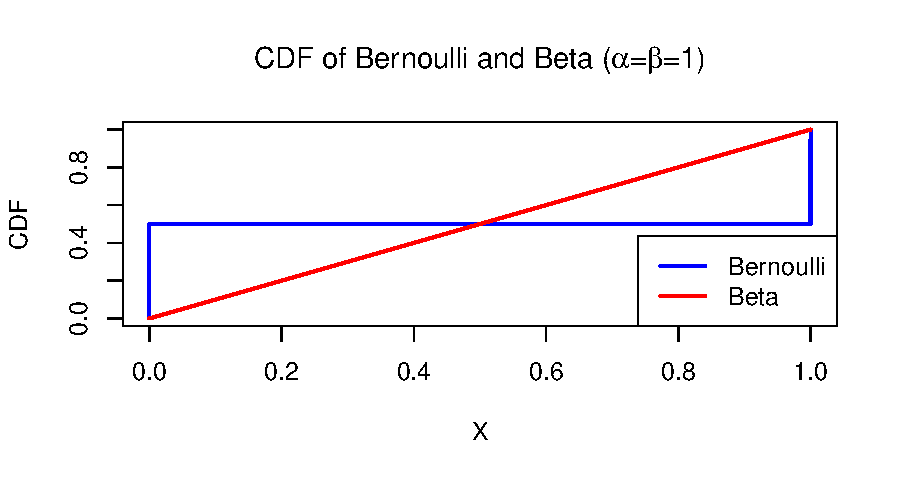
\includegraphics{Homework-01-rmd-for-SMDS-2023-2024_files/figure-latex/unnamed-chunk-27-1} \end{center}

\begin{Shaded}
\begin{Highlighting}[]
\FunctionTok{plot\_bernoulli\_and\_beta}\NormalTok{(}\FloatTok{0.1}\NormalTok{)}
\end{Highlighting}
\end{Shaded}

\begin{center}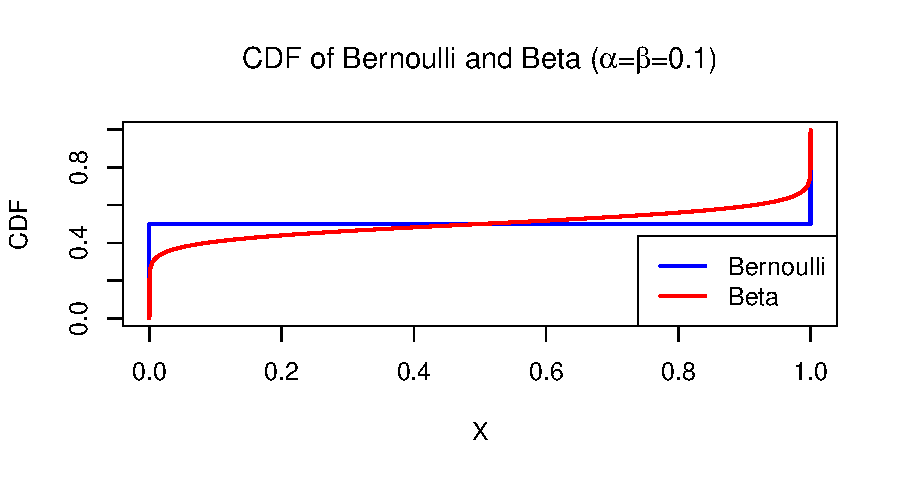
\includegraphics{Homework-01-rmd-for-SMDS-2023-2024_files/figure-latex/unnamed-chunk-28-1} \end{center}

\begin{Shaded}
\begin{Highlighting}[]
\FunctionTok{plot\_bernoulli\_and\_beta}\NormalTok{(}\FloatTok{0.001}\NormalTok{)}
\end{Highlighting}
\end{Shaded}

\begin{center}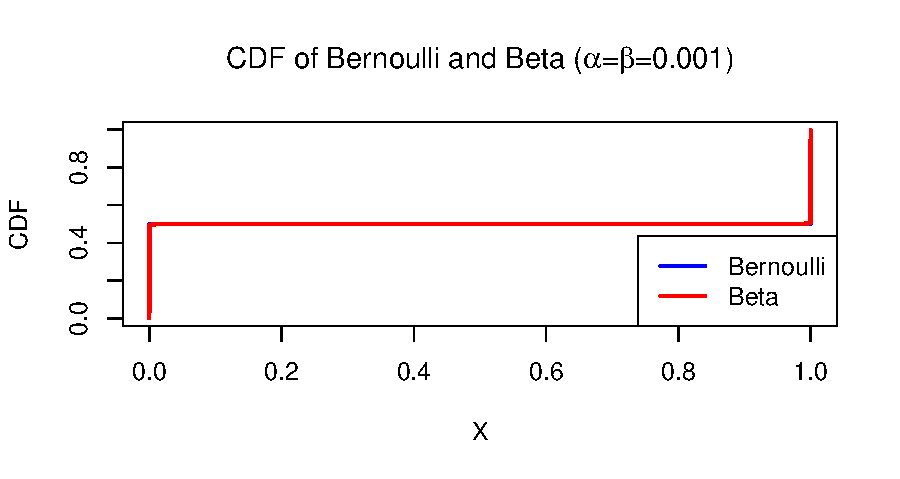
\includegraphics{Homework-01-rmd-for-SMDS-2023-2024_files/figure-latex/unnamed-chunk-29-1} \end{center}

\begin{center}\rule{0.5\linewidth}{0.5pt}\end{center}

© 2023-2024 - Statistical Methods in Data Science and Laboratory II -
2023-2024

\begin{verbatim}
Last update by LT: Fri Apr 26 18:53:02 2024
\end{verbatim}

\end{document}
